\documentclass[english,man]{apa6}

\usepackage{amssymb,amsmath}
\usepackage{ifxetex,ifluatex}
\usepackage{fixltx2e} % provides \textsubscript
\ifnum 0\ifxetex 1\fi\ifluatex 1\fi=0 % if pdftex
  \usepackage[T1]{fontenc}
  \usepackage[utf8]{inputenc}
\else % if luatex or xelatex
  \ifxetex
    \usepackage{mathspec}
    \usepackage{xltxtra,xunicode}
  \else
    \usepackage{fontspec}
  \fi
  \defaultfontfeatures{Mapping=tex-text,Scale=MatchLowercase}
  \newcommand{\euro}{€}
\fi
% use upquote if available, for straight quotes in verbatim environments
\IfFileExists{upquote.sty}{\usepackage{upquote}}{}
% use microtype if available
\IfFileExists{microtype.sty}{\usepackage{microtype}}{}

% Table formatting
\usepackage{longtable, booktabs}
\usepackage{lscape}
% \usepackage[counterclockwise]{rotating}   % Landscape page setup for large tables
\usepackage{multirow}		% Table styling
\usepackage{tabularx}		% Control Column width
\usepackage[flushleft]{threeparttable}	% Allows for three part tables with a specified notes section
\usepackage{threeparttablex}            % Lets threeparttable work with longtable

% Create new environments so endfloat can handle them
% \newenvironment{ltable}
%   {\begin{landscape}\begin{center}\begin{threeparttable}}
%   {\end{threeparttable}\end{center}\end{landscape}}

\newenvironment{lltable}
  {\begin{landscape}\begin{center}\begin{ThreePartTable}}
  {\end{ThreePartTable}\end{center}\end{landscape}}

  \usepackage{ifthen} % Only add declarations when endfloat package is loaded
  \ifthenelse{\equal{\string man}{\string man}}{%
   \DeclareDelayedFloatFlavor{ThreePartTable}{table} % Make endfloat play with longtable
   % \DeclareDelayedFloatFlavor{ltable}{table} % Make endfloat play with lscape
   \DeclareDelayedFloatFlavor{lltable}{table} % Make endfloat play with lscape & longtable
  }{}%



% The following enables adjusting longtable caption width to table width
% Solution found at http://golatex.de/longtable-mit-caption-so-breit-wie-die-tabelle-t15767.html
\makeatletter
\newcommand\LastLTentrywidth{1em}
\newlength\longtablewidth
\setlength{\longtablewidth}{1in}
\newcommand\getlongtablewidth{%
 \begingroup
  \ifcsname LT@\roman{LT@tables}\endcsname
  \global\longtablewidth=0pt
  \renewcommand\LT@entry[2]{\global\advance\longtablewidth by ##2\relax\gdef\LastLTentrywidth{##2}}%
  \@nameuse{LT@\roman{LT@tables}}%
  \fi
\endgroup}


  \usepackage{graphicx}
  \makeatletter
  \def\maxwidth{\ifdim\Gin@nat@width>\linewidth\linewidth\else\Gin@nat@width\fi}
  \def\maxheight{\ifdim\Gin@nat@height>\textheight\textheight\else\Gin@nat@height\fi}
  \makeatother
  % Scale images if necessary, so that they will not overflow the page
  % margins by default, and it is still possible to overwrite the defaults
  % using explicit options in \includegraphics[width, height, ...]{}
  \setkeys{Gin}{width=\maxwidth,height=\maxheight,keepaspectratio}
\ifxetex
  \usepackage[setpagesize=false, % page size defined by xetex
              unicode=false, % unicode breaks when used with xetex
              xetex]{hyperref}
\else
  \usepackage[unicode=true]{hyperref}
\fi
\hypersetup{breaklinks=true,
            pdfauthor={},
            pdftitle={Task instructions modulate unit-decade binding in two-digit number representation},
            colorlinks=true,
            citecolor=blue,
            urlcolor=blue,
            linkcolor=black,
            pdfborder={0 0 0}}
\urlstyle{same}  % don't use monospace font for urls

\setlength{\parindent}{0pt}
%\setlength{\parskip}{0pt plus 0pt minus 0pt}

\setlength{\emergencystretch}{3em}  % prevent overfull lines

\ifxetex
  \usepackage{polyglossia}
  \setmainlanguage{}
\else
  \usepackage[english]{babel}
\fi

% Manuscript styling
\captionsetup{font=singlespacing,justification=justified}
\usepackage{csquotes}
\usepackage{upgreek}



\usepackage{tikz} % Variable definition to generate author note

% fix for \tightlist problem in pandoc 1.14
\providecommand{\tightlist}{%
  \setlength{\itemsep}{0pt}\setlength{\parskip}{0pt}}

% Essential manuscript parts
  \title{Task instructions modulate unit-decade binding in two-digit number
representation}

  \shorttitle{Unit-decade binding in two-digit numbers}


  \author{Thomas J. Faulkenberry\textsuperscript{1}, Alexander Cruise\textsuperscript{2}, \& Samuel Shaki\textsuperscript{2}}

  \def\affdep{{"", "", ""}}%
  \def\affcity{{"", "", ""}}%

  \affiliation{
    \vspace{0.5cm}
          \textsuperscript{1} Tarleton State University\\
          \textsuperscript{2} Ariel University  }

  \authornote{
    \newcounter{author}
    This paper was written in RMarkdown, with code for data analysis
    integrated into the manuscript text. The RMarkdown script and data are
    open and freely available at \url{https://git.io/vhU7z}.\\
    The authors would like to thank Brie Heidingsfelder, Jonathan Herring,
    Heather Hill, and Kate Shaw for their assistance with data collection.
    We would also like to thank Michael Steinborn and an anonymous reviewer
    for their helpful comments on an earlier version of this manuscript.

                      Correspondence concerning this article should be addressed to Thomas J. Faulkenberry, Department of Psychological Sciences, Box T-0820, Tarleton State
University, Stephenville, TX 76401. E-mail: \href{mailto:faulkenberry@tarleton.edu}{\nolinkurl{faulkenberry@tarleton.edu}}
                                    }


  \abstract{Previous studies have found decomposed processes, as well as holistic
processes, in the representation of two-digit numbers. The present study
investigated the influence of task instruction on such processes.
Participants completed both magnitude and parity tasks in one of three
instructional conditions, where they were asked to either consider
two-digit numbers as a whole or to focus on one specific digit. In two
experiments, we found that when participants were asked to consider the
two digits as an integrated number, they always exhibited a unit-decade
compatibility effect, indicating a failure of selective attention on the
digit relevant to the given task. However, the mere presence of the
neighboring digit is not a sufficient condition for the compatibility
effect: when participants were explicitly asked to process a specific
digit, their success/failure to selectively ignore the irrelevant digit
depended on task requirements. Further, computer mouse tracking
indicated that the locus of the compatibility effect was related to late
response-related processing. The results signify the deep involvement of
top-down processes in unit-decade binding for two-digit number
representation.}
  \keywords{Unit-decade compatibility, Selective Attention, Computer mouse tracking,
Top-down processing \\

    
  }





\usepackage{amsthm}
\newtheorem{theorem}{Theorem}
\newtheorem{lemma}{Lemma}
\theoremstyle{definition}
\newtheorem{definition}{Definition}
\newtheorem{corollary}{Corollary}
\newtheorem{proposition}{Proposition}
\theoremstyle{definition}
\newtheorem{example}{Example}
\theoremstyle{definition}
\newtheorem{exercise}{Exercise}
\theoremstyle{remark}
\newtheorem*{remark}{Remark}
\newtheorem*{solution}{Solution}
\begin{document}

\maketitle

\setcounter{secnumdepth}{0}



When a child first learns to associate numerical digits with underlying
numerical quantities, the transition from single-digit numbers to
two-digit numbers presents a challenge. Indeed, two-digit numbers may be
initially treated in such a fashion that the numbers 19 or 91 may not be
discriminated from each other. Later on, however, the child learns about
place value, where the specific location of each digit has its own value
and even name (nine or ninety). With increasing experience, individuals
learn to integrate the separate digits into holistic magnitudes (Klein
et al., 2013; Mussolin \& Noël, 2008). This leads to a natural question:
Are the single digits of a two-digit number indeed merged into an
inseparable internal magnitude code (i.e., holistic processing)? Or is
it perhaps the case that people can flexibly form separate magnitude
representations of the single-digits that comprise a two-digit number
(i.e., decomposed processing)?

\subsection{Models of two-digit number
processing}\label{models-of-two-digit-number-processing}

Early work on this question indicated evidence of holistic processing.
Hinrichs, Yurko, and Hu (1981) asked participants to compare presented
two-digit numbers to a fixed standard (e.g., 55). Hinrichs et al. found
that response times increased as the numerical distance from the
standard decreased. This paralleled the classic numerical distance
effect previously found with single digit numbers (Moyer \& Landauer,
1967) and led Hinrichs et al. to conclude that two digit numbers are
processed holistically as single, integrated quantities. Similarly,
Dehaene, Dupoux, and Mehler (1990) also found that response times
increased as numerical distance decreased, concluding also that symbolic
two-digit numbers must be first encoded into an internal, analogue
representation.

Evidence favoring decomposed processing was reported in the seminal
study by Nuerk, Weger, and Willmes (2001), who found a unit-decade
compatibility effect in comparison of two-digit numbers. When the decade
and unit digits of one number were both smaller (or both larger) than
both digits of the other number (e.g., 23 versus 45), reaction times
(RTs) were faster than if the digits were unit-decade
\emph{incompatible} with each other (e.g.~29 versus 51). This finding
indicates that participants make parallel comparisons of the decade and
unit digits when comparing two-digit numbers, even though the decision
can be made entirely by comparing the decade digits alone (see also
Moeller, Nuerk, \& Willmes, 2009).

The compatibility between the decade and unit digits can also explain
the effect of overall distance that is commonly found in two-digit
number comparison tasks (Dehaene et al., 1990; Hinrichs et al., 1981;
Verguts \& De Moor, 2005). As mentioned earlier, participants tend to
respond faster when deciding whether 68 is larger than 55 than they do
when deciding whether 61 is larger than 55, although a simple decade
comparison is sufficient for deciding in both cases. Indeed, holistic
processing may predict this distance effect, as the overall distance
between 68 and 55 is larger than the overall distance between 61 and 55
(Moyer \& Landauer, 1967). However, the distance effect observed here
may instead be an artifact of unit-decade compatibility. Hence,
measuring the distance effect alone seems to be inconclusive regarding
the nature of two-digit representations (e.g. DeWolf, Grounds, Bassok,
\& Holyoak, 2014; for an extended discussion, see Nuerk, Moeller, Klein,
Willmes, \& Fischer, 2011).

The unit-decade compatibility effect has been replicated in many studies
(Moeller, Klein, Nuerk, \& Willmes, 2013; Moeller et al., 2009; Nuerk \&
Willmes, 2005). Recently, some investigations have focused on examining
the factors that affect the attentional weight of the decade and unit
digits. For example, the unit digit has been found to be more salient
for German participants, who read the unit-digit first (e.g.~24 is said
``four and twenty'\enquote{) than for English, Spanish, or Italian
speakers (Macizo, Herrera, Paolieri, \& Román, 2010; Nuerk, Weger, \&
Willmes, 2005). So, the amount of attention allocated to the two-digit
numerals} components may depend on the structure of the number words
within a language. Also, Castronovo and Crollen (2011) found that the
mode of presentation of the two-digit numbers (e.g., tens first, unit
first, or simultaneously) could determine how much attention is paid to
each component of the two-digit numbers. In addition, Macizo and Herrera
(2011) manipulated the stimulus list by increasing the ratio of
within-decade comparisons, which resulted in a larger unit-decade
compatibility effect. This indicates that even a simple stimulus
manipulation can induce participants to allocate more attention to the
unit-digit.

Finally, in order to test if the processing of two-digit numbers depends
also on task characteristics, Reynvoet, Notebaert, and Van den Bussche
(2011) asked participants to perform either magnitude or parity
judgments on two-digit targets preceded by masked primes. The
briefly-presented primes contained one of the target digits in either a
task-congruent (3\# \(\rightarrow\) 37) or a task-incongruent (\#3
\(\rightarrow\) 37) position. The first digit mainly mediated the
priming effects (e.g., faster RTs for task-congruent primes) in a
magnitude task, presumably because the decade digit has the largest
predictive value when comparing magnitudes (see also Ganor-Stern,
Tzelgov, \& Ellenbogen, 2007; Ratinckx, Brysbaert, \& Fias, 2005). The
opposite pattern was found in the parity task, probably due to the
importance of the unit digit in such a task.

In summary, most recent studies agree that the magnitude of two-digit
numbers is not only represented as one holistic entity, but also
decomposed for its components (units and decades). Participants' failure
to compare the decade digits only while ignoring irrelevant unit digits
(the unit-decade compatibility effect) has served as the key marker in
this notion of decomposed processing (Moeller et al., 2013).

\subsection{Effects of task
instruction}\label{effects-of-task-instruction}

Note that in these previous studies, participants were asked to consider
the two-digit numbers as holistic mathematical units (e.g., to decide if
two-digit number is smaller or larger than 55). The unit-decade
compatibility effect measured their ability to process the two-digit
number as integral mathematical unit (holistically) or not (decomposed
processing). In the present study, however, we tackle the compatibility
effect from another direction: if participants are asked to process
two-digit numbers in a specific decomposed manner, will they be able to
exclusively process the relevant digit, while simultaneously ignoring
the irrelevant digit?

Two recent studies imply that the mere \emph{presence} of adjacent
digits can be enough to elicit automatic processing of the irrelevant
digit. Nuerk, Bauer, Krummenacher, Heller, and Willmes (2005) used an
Eriksen flanker task, in which three identical distractor stimuli
appeared on both left and right sides of a single-digit target. They
found that when distractor stimuli led to the same response as the
target, responses were faster than when they were associated with a
different response, demonstrating that participants processed the
magnitude of the irrelevant adjacent digit. Similarly, Kallai and
Tzelgov (2012) presented single-digit numbers as three digit strings
with zeros in two of three positions. They manipulated the position of
the nonzero digit, presenting it in either the hundreds position, the
decade position, or the unit position. Even though participants were
asked to ignore the zeros, Kallai and Tzelgov found that the position of
the nonzero digit had a significant effect on response patterns, even
though the position was irrelevant to the task. Once again, such a
result indicates that participants may automatically form
representations of the magnitude of multiple digits.

Note that both of the above studies specifically used a magnitude task.
In addition, the location of the adjacent digit(s) was not controlled.
For example, the distractor stimuli in Nuerk et al. (2005) were
presented on both the left and right sides of the target. Therefore,
these studies do not allow us to fully investigate the influence of
specific task characteristics, or the potential interaction between task
(i.e., magnitude or parity) and the side (left or right) of the adjacent
digit. Nevertheless, these studies imply that at least in \emph{some}
cases, (a) the mere presence of digits next to each other in a
vertically-aligned fashion is sufficient for participants to process
them automatically even without an explicit instruction, and (b) that
participants are aware of the place-value of a digit even if it is
irrelevant to the task.

To summarize, systematic studies into the influence of task instructions
on unit-decade binding in two-digit numbers remain scarce, and the
debate on its specific role is ongoing. In our study, we aimed to
explore the effect of \emph{task instructions} on the processing of
two-digit numbers by using the unit-decade compatibility effect as a
marker of decomposed processing. Our second aim was to examine the
flexibility and boundary conditions under which these binding effects
appear. Precisely, we asked whether the presence of two digits next to
each other was sufficient for participants to treat them as a two-digit
number. Or, perhaps, is it necessary to explicitly define our stimuli as
a two-digit number (through task instructions) in order for such
unit-decade binding to occur?

Why should specific task instructions matter? Evidence in support of
instruction-based modulation of response activation comes from studies
showing that specific stimulus-response mappings induced by task
instructions can trigger response tendencies in an irrelevant task
(e.g., Cohen-Kdoshay \& Meiran, 2007; Liefooghe, De Houwer, \& Wenke,
2013; Wenke \& Frensch, 2005; Wenke, Gaschler, \& Nattkemper, 2005).
Thus, we expect that task instructions might not only serve to associate
digits with specific responses in a single task, but also co-activate a
response based on the neighboring digit, thus effectively binding the
components of two-digit number into a single, unitary representation.
This hypothesis is predicted directly by a dual-route model which
assumes that task-relevant and task-irrelevant information are processed
in parallel by two independent routes (e.g., De Jong, Liang, \& Lauber,
1994; Kornblum, Hasbroucq, \& Osman, 1990; Zorzi \& Umiltà, 1995).

The mechanism for this dual-route model is as follows. One route (a
\emph{conditional route}) processes task-relevant stimulus information
based on current task instructions, which determine how stimulus events
and actions are bound together in given situation. For example, in a
parity judgment task, task instructions will specify that if a number is
even, the participant should press the left button, and conversely, if a
number is odd, one press the right button. Thus, the task instruction
produces two stimulus-response mappings: \enquote{even = right} and
\enquote{odd = left}. At the same time, an \emph{unconditional route}
processes task-irrelevant stimulus information (e.g., an irrelevant
flanker digit) and primes its associated motor response. According to
the model, response duration depends on the degree to which the
instruction-induced SR mappings (associated with the two routes) are
shared by the two competing stimuli. That is, if the two routes converge
on the same response, processing is \emph{facilitated} (i.e., fast RTs),
whereas if the two routes activate opposing responses, processing is
\emph{inhibited} (i.e., slow RTs). For a concrete example, consider the
number 13. If participants are asked to make a parity judgment of the
unit digit only (i.e., the \enquote{3}), the dual-route model predicts
that participants will be relatively quick to make the judgment, as both
the conditional route (mapping the stimulus \enquote{3} to the response
\enquote{press left button}) and the unconditional route (mapping the
irrelevant stimulus \enquote{1} to the response \enquote{press left
button}) converge to the same response. However, if the number 23 is
presented, we may expect an interference effect, thus slowing down
response times. This is because the conditional route maps the task
relevant digit \enquote{3} to the response \enquote{press left button}
(because 3 is odd), but the unconditional route maps the irrelevant
digit \enquote{2} to the response \enquote{press right button} (because
2 is even).

However, this prediction assumes that participants implicitly place
equal weight on the information carried by the two digits. For example,
in a parity judgment, only the unit digit is relevant to the decision
(e.g., the even/odd status of 23 is determined \emph{completely} by the
unit digit 3). Thus, in the context of a parity task on unit digits, the
decade digit is irrelevant to the decision (even in the context of a
two-digit number), and thus the activation of the unconditional route
may be reduced. As a result, any processing in the unconditional route
may not weigh as heavily on the final decision. Thus, the interference
between response mappings may be reduced, reflecting a role for top-down
control in the dual-route model. At present, the exact nature of these
response conflicts in two-digit number representation is not clear; the
need for such descriptive data forms the basis for the present study.

\subsection{The present study}\label{the-present-study}

In the present study, we sought to understand the conditions under which
task instructions can modulate unit-decade binding in two digit numbers.
To this end, we asked participants to separately perform magnitude and
parity tasks with two-digit numbers. Within each task, we gave three
different types of instructions: \emph{overall}, \emph{decade-only}, and
\emph{unit-only}. In the overall condition, the participants' task was
to consider the stimuli as a \enquote{two-digit number}. Thus, for the
magnitude task, the specific instruction was to decide if the two-digit
number was smaller or larger than 55. For the parity task, the specific
instruction was to decide if the two-digit number was odd or even. The
overall condition served as a benchmark for our other critical
decomposed conditions. In the two decomposed instructional conditions,
participants were explicitly instructed to pay attention to only the
decade or the unit digit. In the magnitude task, they were to decide if
the single relevant digit was smaller/larger than 5, and in the parity
task, they were to decide whether the single digit was odd/even.
Importantly, in these decomposed instructional conditions, the adjacent
digit always served as a task-irrelevant stimulus and was unassociated
with the correct response required for the target digit. Hence, we were
especially interested in observing whether participants could ignore the
irrelevant digit and focus their attention exclusively on the target
digit.

In our experiments, we explicitly manipulated the \emph{congruency} of
the digits in each stimulus. The definitions of congruent/incongruent
depended on task. For example, in the parity task, trials were congruent
when both the task-relevant and task-irrelevant digits required the same
response (i.e., both digits odd or both even, such as 37 or 46). Parity
trials were incongruent when the two digits required opposite responses
(i.e., one digit odd and the other even, such as 78). Congruency on the
magnitude task was defined similarly; trials were congruent when both
digits required the same response (i.e., both digits smaller or larger
than 5, such as 23 or 78) and incongruent when digits resulted in
opposite responses (i.e., one digit smaller than 5 and the other larger,
such as 28 or 73). In light of this congruency manipulation, we
hypothesized that our instructional conditions (overall, decade-only, or
unit-only) would modulate attentional focusing towards the irrelevant
digit only when the irrelevant digit is relevant for completion of a
specific task. As a consequence, in the magnitude task, we predict that
greater interference will occur when the distractor is in the decade
position (i.e., when participants are asked to pay attention to only the
unit digit). In contrast, in the parity task, we expect more pronounced
interference from neighbors in the unit position (i.e., when
participants are asked to pay attention to only the decade digit).

We tested these predictions in two experiments that used similar stimuli
and procedures, but we varied the response mode. In Experiment 1,
participants categorized parity/magnitude status of a target digit using
left-right keypress responses, from which we measured response times
(RTs) and error rates. In Experiment 2, we used computer mouse tracking
(Freeman \& Ambady, 2009; Freeman, Dale, \& Farmer, 2011; Spivey,
Grosjean, \& Knoblich, 2005) to record the kinematics of participants'
hand movements as they categorized parity/magnitude by moving a mouse
cursor from a central \enquote{start} area to a target areas positioned
in the upper left or right corner of the screen. Such an approach has
been used in several recent studies in numerical cognition (Erb, Moher,
Song, \& Sobel, in press; Faulkenberry, 2014, 2016; Faulkenberry,
Cruise, \& Shaki, 2017; Faulkenberry, Cruise, Lavro, \& Shaki, 2016;
Faulkenberry, Hartmann, \& Witte, in press; Faulkenberry, Montgomery, \&
Tennes, 2015; Santens, Goossens, \& Verguts, 2011; Song \& Nakayama,
2008). Importantly, this approach allowed us two empirical advantages.
First, we were able to record the streaming \(x,y\)-coordinates of the
computer mouse movements during the decision process. Any systematic
spatial deviations between mouse trajectories that arise from our
experimental manipulations would provide evidence of competition between
response options that cannot be easily detected from patterns of RTs
alone. Second, computer mouse tracking gives us a means to record
response times in a decomposed fashion, breaking the total RT into
components of \emph{initiation time} (the time elapsed between stimulus
presentation and initial mouse movement) and \emph{movement time}
(reflecting the actual duration of mouse movement). This provides a
potentially sensitive method for further discerning the locus of any RT
patterns obtained in Experiment 1, which will allow us to effectively
test the generality of our predictions across different response modes.

\section{Experiment 1}\label{experiment-1}

\subsection{Method}\label{method}

\subsubsection{Participants}\label{participants}

Sixteen students (6 male, 10 female, mean age 22.1 years, SD = 2.03
years) from Ariel University participated in three experimental sessions
in exchange for partial course credit. Two of the male participants
reported that they were left handed. All participants were born in
Israel and were Hebrew-English bilinguals.

\subsubsection{Stimuli and apparatus}\label{stimuli-and-apparatus}

The stimulus set consisted of all two-digit numbers in the range 11-99,
excluding numbers with 5 or 0 in it (e.g., 40 or 51). These 64 two-digit
numbers were replicated, resulting in 128 trials in a single block (see
below for design). Half of the stimuli were smaller than 55 and half
were larger than 55. Half of the numbers were odd and the other half
were even. Finally, the number of congruent and incongruent numbers was
equal in both tasks. The stimuli were presented in their Arabic form and
appeared in black Times New Roman font (size 30) at the center of the
screen on a white background of a 17-in. (43 cm, 1024 X 768 pixel
resolution) monitor. Responses were made on a standard QWERTY keyboard,
with all keys covered except A (left hand responses) and L (right hand
responses). Response times and accuracy were recorded with SuperLab 2.0.

\subsubsection{Design}\label{design}

All independent variables were manipulated within-subjects. The 128
number stimuli described above were repeated (randomly without
replacement) in 12 different blocks, each of which was defined via the
factorial manipulation of three independent variables, which we describe
as follows. There were three instructional conditions where we
manipulated the target (overall, decade, unit) and two different task
orders (magnitude task first, parity task first), all of which were
performed under two different response rules, depending on task
(\enquote{small=left} or \enquote{small=right} for the magnitude task,
and \enquote{even=left} or \enquote{even=right} for the parity task).
All together, this factorial combination (12 blocks of 128 trials)
resulted in 1536 trials in total per participant.

Participants performed these 12 blocks of trials in three separate
experimental sessions, each separated by one week. In the first session,
participants completed four blocks (512 trials) of the \enquote{overall}
instructional condition, performing both the magnitude and parity tasks
under the two different response rules. Then, in each of the two
subsequent sessions, participants repeated this design for both the
\enquote{decade} and \enquote{unit} instructional conditions, completing
4 experimental blocks each day (512 trials). Note that the two response
rules for each task (parity, magnitude) were always done in two
consecutive blocks. The task order, the decade and unit conditions
order, and the order of the response rules were counterbalanced across
participants, but were kept fixed along the experiment for each
participant. Finally, the order of stimuli was randomized within each
block.

\subsubsection{Procedure}\label{procedure}

Data were collected in a dimly lit room with the participant seated
approximately 50 cm from the center of the screen. In each trial, a
fixation cross appeared for 500 ms on a blank screen and was then
followed by a randomly selected two-digit number. In the overall
condition, the participant's task was to decide if the two-digit number
is smaller or larger than 55 (magnitude task) or if the two-digit number
is odd or even (parity task). In the decade and the unit conditions, the
participant's task was to decide if the relevant digit (leftmost digit
or rightmost digit) is smaller or larger than five (magnitude task), or
if the relevant digit is odd or even (parity task). The left/right
response keys served for odd/even and smaller/larger responses,
according to the previously agreed response rule. Each stimulus number
stayed on the screen until a response was made, and the next trial began
500 ms later.

A planned break of 15 minutes between tasks was given, while a short 5
minute break separated the two consecutive blocks of response rules
within each task. Each session took approximately 50 minutes to
complete, and approximately one week separated between the three
different sessions.

\subsection{Results}\label{results}

Participants completed a total of 24576 experimental trials. Two trials
were inexplicably not recorded in the data file. From the remaining
24574 trials, we initially discarded 471 outlier trials using the
following procedure. For each factorial combination of participant and
experimental condition (i.e., each \emph{design cell}), we computed the
mean and standard deviation of the distribution of response times for
correct trials. Then, we discarded any trial for which the response time
satisfied one of two conditions: (a) the RT was less than 200 ms; or (b)
the RT was larger than the mean RT plus 2.5 standard deviations, where
mean and standard deviation were calculated for the specific design cell
from whence the trial originated. After this cleaning procedure, we
retained 98.10\% of the original trials for our data analysis. Across
the 16 participants, the percentage of outliers for each participant
ranged between 0.91\% and 2.99\% (mean outlier rate = 1.90\%).

Unit-decade congruency was defined in a conceptually similar way for
both magnitude and parity tasks: a two-digit number was defined as
\emph{congruent} if both decade and unit digits led to an identical
response. The number was defined as incongruent if the digits yielded
conflicting responses. For instance, the two-digit number 34 was
considered as congruent in the magnitude task (since both decade and
unit are less than 5), but as an incongruent in the parity task (since 3
is odd, but 4 is even).

\begin{table}[tbp]
\begin{center}
\begin{threeparttable}
\caption{\label{tab:exp1table}Descriptive statistics for performance measures in Experiment 1}
\begin{tabular}{llccc}
\toprule
 &  & \multicolumn{2}{c}{RT (ms)}  &\\
\cmidrule(r){3-4}
Condition & \multicolumn{1}{c}{Congruency} & \multicolumn{1}{c}{Mean} & \multicolumn{1}{c}{SD} & \multicolumn{1}{c}{Error rate (\%)}\\
\midrule
{\it Magnitude task} &  &  &  & \\
Overall & congruent & 618.65 & 233.31 & 1.84\\
 & incongruent & 643.11 & 248.12 & 2.59\\
Decade & congruent & 575.99 & 194.98 & 2.23\\
 & incongruent & 580.28 & 198.48 & 2.73\\
Unit & congruent & 589.21 & 225.96 & 1.89\\
 & incongruent & 610.35 & 216.12 & 4.11\\
{\it Parity task} &  &  &  & \\
Overall & congruent & 637.75 & 218.14 & 2.10\\
 & incongruent & 656.11 & 204.61 & 3.81\\
Decade & congruent & 613.04 & 206.81 & 7.59\\
 & incongruent & 653.48 & 230.16 & 12.08\\
Unit & congruent & 607.39 & 220.85 & 3.94\\
 & incongruent & 620.64 & 217.75 & 4.27\\
\bottomrule
\addlinespace
\end{tabular}
\begin{tablenotes}[para]
\textit{Note.} Mean RT and SD were computed for correct trials only.
\end{tablenotes}
\end{threeparttable}
\end{center}
\end{table}

\begin{figure}
\centering
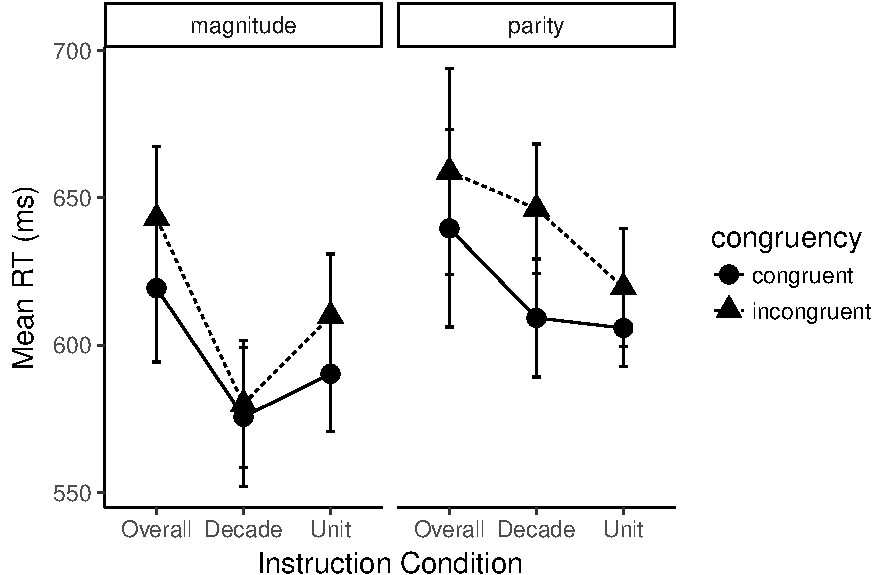
\includegraphics{paper_files/figure-latex/exp1-1.pdf}
\caption{\label{fig:exp1}Mean RTs for Experiment 1, presented as a function
of congruency (congruent, incongruent), instruction condition (overall,
decade only, unit only), and task (magnitude, parity). Error bars
represent within-subject 95\% confidence intervals as recommended by
Morey (2008).}
\end{figure}

\subsubsection{Response time analysis}\label{response-time-analysis}

We first analyzed response times on correct trials. To this end, we
removed 988 error trials (overall error rate = 4.10\%). Distributions of
response times for each factorial combination of participant and
experimental condition were collapsed to a single point by computing the
mean RT, upon which we performed analyses of variance (ANOVA) to test
the effects of our experimental manipulations.

In order to compare the congruency effect between tasks and the
different instruction conditions we first ran a two-way ANOVA for mean
RTs in the overall condition with factors of task and congruency only
(see Table \ref{tab:exp1table}). We found a main effect of congruency,
\(F(1, 15) = 13.23\), \(p = .002\), \(\eta^2_p = .469\). As shown in
Figure \ref{fig:exp1}, responses to incongruent numbers in the overall
condition were slower for both the magnitude and parity tasks. Neither
the main effect of task {[}\(F(1, 15) = 0.84\), \(p = .373\){]} nor the
interaction between task and congruency {[}\(F(1, 15) = 0.14\),
\(p = .711\){]} reached significance. Hence, the compatibility effect
did not differ between the magnitude and parity tasks.

We next aimed to check if the compatibility effect differed between the
decade and unit conditions. To this end, we ran another ANOVA for mean
RTs with independent variables of task, congruency, and the two crucial
instructional conditions (decade only, unit only). There was a
significant main effect of task, \(F(1, 15) = 8.86\), \(p = .009\),
\(\eta^2_p = .371\). On average, the magnitude task was 34.18 ms faster
than the parity task. In addition, there was a significant main effect
of congruency, \(F(1, 15) = 34.35\), \(p < .001\), \(\eta^2_p = .696\).
Responses to incongruent numbers were 19.11 ms slower than responses to
congruent numbers. There was no main effect of instructional condition,
\(F(1, 15) = 0.16\), \(p = .695\), \(\eta^2_p = .011\).

There was also an interaction between task and condition,
\(F(1, 15) = 8.45\), \(p = .011\), \(\eta^2_p = .360\), and this
interaction depended on congruency condition, as signified by the
significant three-way interaction between task, instruction condition,
and congruency, \(F(1, 15) = 12.98\), \(p = .003\), \(\eta^2_p = .464\).
As shown in Figure \ref{fig:exp1}, when participants were asked to focus
their attention on the decade digit and ignore the unit digits, there
was no effect of congruency in the magnitude task, \(t(15) = 0.70\),
\(p = .495\). However, there was a large effect of congruency in the
parity task, \(t(15) = 6.53\), \(p < .001\), indicating that
participants suffered from intrusions from the irrelevant unit digit. By
contrast, when participants were asked to pay attention to only the
units digit, a large congruency effect appeared in the magnitude task,
\(t(15) = 4.35\), \(p = .001\), but the congruency effect was
nonsignificant in the parity task, \(t(15) = 1.89\), \(p = .079\). No
other terms in the ANOVA model were statistically significant.

\subsubsection{Error analysis}\label{error-analysis}

We also analyzed how error rates differed as a function of our
experimental manipulations. We first performed a two-way ANOVA for error
rates in the overall condition with factors of task and congruency only.
As with response times, there was a significant main effect of
congruency, \(F(1, 15) = 5.48\), \(p = .034\), \(\eta^2_p = .267\). As
can be seen in Table \ref{tab:exp1table}, error rates were larger on
incongruent trials compared to congruent trials. Neither the main effect
of task {[}\(F(1, 15) = 0.97\), \(p = .340\){]} nor the interaction
between task and congruency {[}\(F(1, 15) = 1.86\), \(p = .193\){]}
reached significance.

We next performed an ANOVA for error rates with factors of task,
congruency, and instructional condition (decade only, unit only). There
was a significant main effect of task, \(F(1, 15) = 5.39\),
\(p = .035\), \(\eta^2_p = .264\). As can be seen in Table
\ref{tab:exp1table}, participants made more errors in the parity task
than they did in the magnitude task. There was also a significant main
effect of congruency, \(F(1, 15) = 13.22\), \(p = .002\),
\(\eta^2_p = .469\), indicating that error rates were larger for
incongruent trials than for congruent trials. Finally, there was a
significant three-way interaction between task, congruency, and
instructional condition, \(F(1, 15) = 10.37\), \(p = .006\),
\(\eta^2_p = .409\), driven primarily by the large error rates (and
large congruency effect) for decade-only trials in the parity task. No
other terms in the ANOVA model were statistically significant.

\subsection{Discussion}\label{discussion}

The pattern of unit-decade compatibility effects (which we term as
\emph{congruency} effects here) appears to depend heavily on specific
task characteristics. For the magnitude task, we found a congruency
effect in the overall condition but not in the decade-only condition of
the magnitude task. Since the same stimulus set was presented in both
conditions, the only difference was whether we asked participants to
compare the two-digit number to 55 (the overall condition) or to compare
the left digit to 5 (the decade condition). In both conditions,
participants could have successfully completed the task by focusing only
on the leftmost digit. However, by asking participants to compare to 55
(and thus implicitly defining the two adjacent digits as a two-digit
number), we induced participants to process the irrelevant digit as
well, thus resulting in the observed congruency effect.

A different pattern emerged in the parity task. There, we again found a
congruency effect in the overall condition but not in the \emph{unit}
condition. Again, the same stimulus set was presented in both conditions
and the only difference was whether we instructed the participant to
classify the parity of the two-digit number (the overall condition) or
of the rightmost digit (the unit condition). In each case, the task
could have been successfully completed by attending to only the
rightmost digit. However, the congruency effect was found in the overall
condition but not in the unit condition.

So far, these findings can be interpreted as follows. As in past
studies, when participants were instructed to consider the two digits as
a holistic two-digit number (the overall condition), they automatically
processed both digits, as was demonstrated by the observed unit-decade
compatibility effect in both magnitude and parity tasks. However, such a
failure of the selective attention was not always found when
participants were explicitly instructed to consider the two adjacent
digits in a decomposed manner (decade and unit conditions). The absence
of the equivalent Stroop-like interference effect in the decade
condition of the magnitude task and the unit condition of the parity
task indicate that processing of the irrelevant adjacent digit is not
always obligatory. Indeed, it appears that specific task characteristics
can modulate the unit-decade binding processes in two-digit number
representation.

\section{Experiment 2}\label{experiment-2}

In Experiment 2, we tested the generality of our findings by replicating
the basic procedure of Experiment 1, but instead of using button
presses, we had participants indicate their decisions via a computer
mouse click. This allowed us additionally to track participants' hand
movements during their decisions, giving a window into the evolution of
the decision process (Freeman \& Ambady, 2009; Freeman et al., 2011;
Spivey et al., 2005). As mentioned earlier, this approach has been
recently used in several studies to investigate the temporal dynamics of
numerical processing (see Faulkenberry et al., in press for a review).

\subsection{Method}\label{method-1}

\subsubsection{Participants}\label{participants-1}

Sixty undergraduate students (8 male, 52 female, mean age 24.1 years,
SD=5.2 years) participated in this experiment in exchange for partial
course credit in their psychology courses. One participant was removed
from further analysis due to an experimenter error during data
collection, leaving 59 participants total. The experiment was reviewed
and approved by the institutional review board at Tarleton State
University.

\subsubsection{Apparatus}\label{apparatus}

The experiment was coded and delivered using the MouseTracker software
package (Freeman \& Ambady, 2010). All experimental trials were
presented on a 20 inch iMac desktop computer with a screen resolution of
1,280 x 1,024 pixels and a refresh rate of 60 Hz. Input was captured via
a Dell optical mouse connected via USB. Participants were seated in a
manner such that there was a distance of approximately 60 cm between the
computer display and the participants' eyes. Participants were
instructed to hold the computer mouse in a manner which was comfortable.
All participants held the mouse in the right hand, positioned slightly
to the right of center on the computer table.

We ran the MouseTracker program on the iMac using a virtual Windows XP
environment via Parallels. As per the recommendations of M. H. Fischer
and Hartmann (2014), we disabled the \enquote{dynamic acceleration}
option and lowered the speed of the mouse movements on the screen to the
second-lowest possible speed in the mouse settings dialog. This is done
to prevent quick and erratic mouse movements, resulting in a smooth and
more reliable record of participants' hand movements. The resulting
displacement ratio of the mouse to screen movement was 1 cm to 100
pixels.

\subsubsection{Stimuli and procedure}\label{stimuli-and-procedure}

We designed computer mouse tracking versions of the same two-digit
number tasks described in Experiment 1, with stimuli consisting of the
64 two-digit numbers described in Experiment 1. Participants completed a
magnitude task and a parity task according to one of three randomly
assigned instructional conditions: overall (\(n=19\)), decade-only
(\(n=20\)), or unit-only (\(n=20\)). Participants in the overall
condition were told that they would be presented with a single two-digit
number. Participants in the decade-only condition were presented with
\enquote{two digits next to each other}, and were instructed to pay
attention to only the \emph{left} digit. Participants in the unit-only
condition were given similar instructions, except that they were
instructed to pay attention to only the \emph{right} digit.

All participants completed 256 experimental trials, consisting of a
block of 128 trials of a magnitude task and block of 128 trials of a
parity task. These task blocks were completed in counterbalanced order.
Half of the participants began with the magnitude task block, whereas
the other half began with the parity task block. For participants in the
overall condition, the magnitude task required participants to choose,
as quickly as possible, whether the presented two-digit number was less
than 55 or greater than 55. Participants in the decade-only and
unit-only conditions were instructed to choose whether the relevant
single digit (left or right, respectively) was less than 5 or greater
than 5. The parity task required participants to choose whether the
presented number was even or odd. For participants in the overall
condition, they were instructed to decide whether the two-digit number
was even or odd, whereas participants in the decade-only and unit-only
conditions were instructed to decide whether the relevant single digit
(left or right, respectively) was even or odd.

Each trial began with a blank screen presented for 500 ms, followed by a
screen that displayed the appropriate response labels at the top left
and right of the screen, respectively, as well as a single
\enquote{Start} button at the bottom center of the screen. Each response
label was presented in Arial font with point size 24. Response labels
depended on task; for the magnitude task, the response labels were
\enquote{Small} and \enquote{Large}, whereas for the parity task, the
response labels were \enquote{Even} and \enquote{Odd}. Within a
single-task block (128 trials), the left-right ordering of the response
labels was switched halfway through the block (i.e., after the
completion of 64 trials).

Once the \enquote{Start} button was pressed, one of the 64 stimulus
numerals appeared in the center of the screen, presented in Times New
Roman font with point size 30. Participants then clicked on the correct
response option; while doing so, the software recorded the streaming
\((x, y)\) coordinates of the computer mouse approximately 63 times per
second. The left-right position of the correct response option was
counterbalanced across trials within each block.

For incorrect responses, the program displayed an \enquote{X} for 2000
ms. To ensure that trajectories reflected online processing,
participants were encouraged to begin their movements as early as
possible and were warned if initiated movement later than 400 ms
following number pair presentation. This instruction is customarily
included in mousetracking studies so that trajectories reflect the
dynamics of a decision process rather than simply reflecting the
kinematics of a response choice after the choice has already been made
(Freeman \& Ambady, 2009; Spivey et al., 2005).

In total, participants completed two blocks of each of two tasks,
resulting in 4 repetitions of the 64 number stimulus set. Thus, each
participant completed 256 experimental trials in a single 30 minute
session.

\subsection{Results}\label{results-1}

Participants completed a total of 15104 experimental trials. We
initially discarded 401 outlier trials using the procedure described in
Experiment 1. After this cleaning procedure, we retained 97.30\% of the
original trials for further analysis. Across the 59 participants, the
percentage of outliers for each participant ranged between 1.17\% and
5.47\% (mean outlier rate = 2.63\%).

\begin{table}[tbp]
\begin{center}
\begin{threeparttable}
\caption{\label{tab:exp2table}Descriptive statistics for performance measures in Experiment 2}
\begin{tabular}{llccccc}
\toprule
 &  & \multicolumn{2}{c}{MT (ms)} & \multicolumn{2}{c}{Init (ms)}  &\\
\cmidrule(r){3-4} \cmidrule(r){5-6}
Condition & \multicolumn{1}{c}{Congruency} & \multicolumn{1}{c}{Mean} & \multicolumn{1}{c}{SD} & \multicolumn{1}{c}{Mean} & \multicolumn{1}{c}{SD} & \multicolumn{1}{c}{Error rate (\%)}\\
\midrule
{\it Magnitude task} &  &  &  &  &  & \\
Overall & congruent & 958.76 & 244.85 & 156.39 & 109.58 & 0.00\\
 & incongruent & 987.85 & 258.71 & 148.56 & 105.00 & 0.67\\
Decade & congruent & 1,043.46 & 257.44 & 122.89 & 111.00 & 0.00\\
 & incongruent & 1,038.94 & 252.17 & 119.06 & 107.20 & 3.77\\
Unit & congruent & 1,009.30 & 237.90 & 112.18 & 94.87 & 0.00\\
 & incongruent & 1,032.61 & 229.18 & 107.14 & 86.59 & 2.87\\
{\it Parity task} &  &  &  &  &  & \\
Overall & congruent & 986.95 & 222.29 & 152.57 & 110.83 & 0.00\\
 & incongruent & 1,019.06 & 232.76 & 150.96 & 109.01 & 0.76\\
Decade & congruent & 1,086.19 & 277.69 & 139.14 & 129.57 & 0.00\\
 & incongruent & 1,124.68 & 295.47 & 137.05 & 129.18 & 3.21\\
Unit & congruent & 1,021.90 & 250.66 & 119.67 & 110.71 & 0.00\\
 & incongruent & 1,048.96 & 261.50 & 116.46 & 112.61 & 1.52\\
\bottomrule
\addlinespace
\end{tabular}
\begin{tablenotes}[para]
\textit{Note.} MT = movement time; Init = initiation time.
\end{tablenotes}
\end{threeparttable}
\end{center}
\end{table}

\subsubsection{Time analyses}\label{time-analyses}

For each trial, the MouseTracker software recorded two time-based
performance measures. The first of these, reaction time (RT), is defined
as the total time elapsed from when the participant began a trial by
clicking the START button until the target mouse click. The second
measure, initiation time (Init), is defined as the time elapsed from the
initial mouse click of the START button until the onset of mouse
movement. From these two measures, we calculated movement time (MT),
which indexes the temporal duration of mouse movement, by subtracting RT
- Init on each trial. We present the summary statistics for these two
measures (MT and Init) in Table \ref{tab:exp2table}.

\begin{figure}
\centering
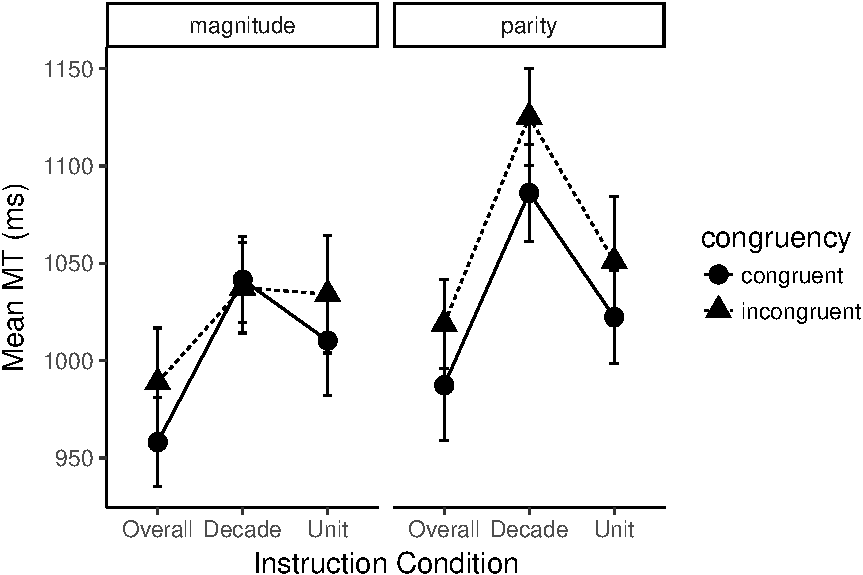
\includegraphics{paper_files/figure-latex/exp2-mt-1.pdf}
\caption{\label{fig:exp2-mt}Mean computer mouse movement times (MTs) in
Experiment 2, presented as a function of congruency (congruent,
incongruent), instruction condition (overall, decade only, unit only),
and task (magnitude, parity). Error bars represent within-subject 95\%
confidence intervals as recommended by Morey (2008).}
\end{figure}

\paragraph{Movement times}\label{movement-times}

Similar to the approach taken in Experiment 1, we aimed to first compare
the congruency effect between tasks and the different instruction
conditions by first conducting a two-way ANOVA on the mean movement
times (MTs) for the overall condition with factors of task and
congruency only. We found a main effect of congruency,
\(F(1, 18) = 40.43\), \(p < .001\), \(\eta^2_p = .692\). As shown in
Figure \ref{fig:exp2-mt}, incongruent numbers in the overall condition
resulted in longer mouse movement durations for both the magnitude and
parity tasks. Neither the main effect of task {[}\(F(1, 18) = 2.22\),
\(p = .154\), \(\eta^2_p = .110\){]} nor the interaction between task
and condition {[}\(F(1, 18) = 0.01\), \(p = .935\){]} were significant.

Next we aimed to test whether the congruency effect differed between the
decade and unit conditions. We submitted mean MTs to a three-way ANOVA
with independent variables of task, congruency, and instructional
condition (restricted to the decade only and unit only conditions).
Overall, the results were similar to those with RTs in Experiment 1.
There was a significant main effect of task, \(F(1, 38) = 7.91\),
\(p = .008\), \(\eta^2_p = .172\), indicating that MTs in the parity
task were longer than those in the magnitude task. There was also a
significant main effect of congruency, \(F(1, 38) = 24.42\),
\(p < .001\), \(\eta^2_p = .391\), where MTs for incongruent numbers
were longer than MTs for congruent numbers. There was no main effect of
instructional condition, \(F(1, 38) = 1.11\), \(p = .299\),
\(\eta^2_p = .028\).

The interaction between task and instructional condition that we
observed in Experiment 1 with RTs did not reach significance with MTs in
Experiment 2, \(F(1, 38) = 3.23\), \(p = .080\), \(\eta^2_p = .078\).
However, there was an interaction between task and congruency,
\(F(1, 38) = 24.42\), \(p < .001\), \(\eta^2_p = .391\), and this
interaction depended on instructional condition, as signified by a
significant three-way interaction, \(F(1, 38) = 6.10\), \(p = .018\),
\(\eta^2_p = .138\). As shown in Figure \ref{fig:exp2-mt}, when
participants were asked to focus only on the decade digit and ignore the
unit digit, there was no effect of congruency on MTs in the magnitude
task, \(t(19) = -0.59\), \(p = .565\). However, we did observe a large
congruency effect in the parity task, \(t(19) = 3.54\), \(p = .002\),
indicating a failure of selective attention on the parity task. In
contrast to Experiment 1, when we asked participants to pay attention to
only the units digit, a large congruency effect appeared in both the
magnitude task, \(t(19) = 3.14\), \(p = .005\), and the parity task,
\(t(19) = 4.15\), \(p = .001\). No other terms in the ANOVA model were
statistically significant.

\begin{figure}
\centering
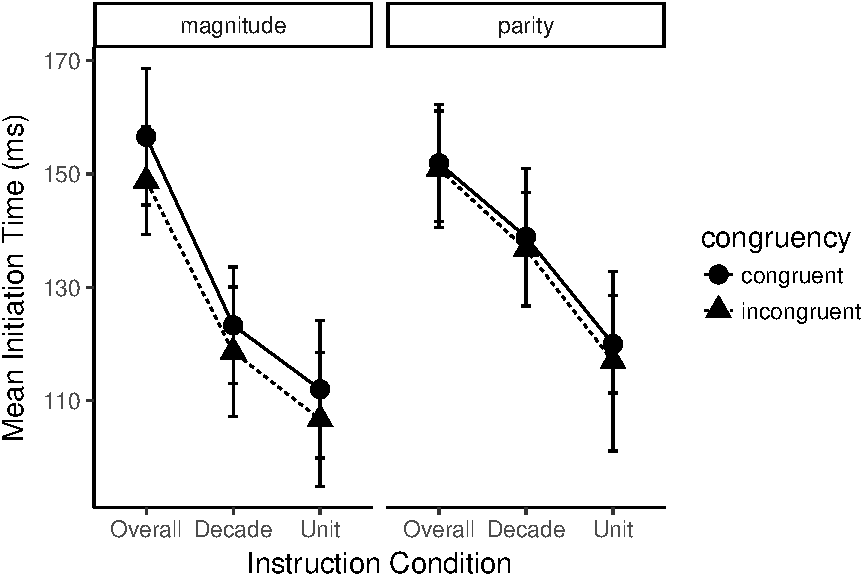
\includegraphics{paper_files/figure-latex/exp2-init-1.pdf}
\caption{\label{fig:exp2-init}Mean mouse initiation times as a function of
congruency (congruent, incongruent), instruction condition (overall,
decade only, unit only), and task (magnitude, parity). Error bars
represent within-subject 95\% confidence intervals as recommended by
Morey (2008).}
\end{figure}

\paragraph{Initiation times}\label{initiation-times}

Mouse initiation times were submitted to a three-way ANOVA with factors
of congruency, task, and instruction condition. There was a significant
main effect of congruency, \(F(1, 56) = 6.58\), \(p = .013\),
\(\eta^2_p = .105\), with faster initiation times on incongruent trials.
The effect of instructional condition on initiation time was not
statistically significant, \(F(2, 56) = 2.85\), \(p = .066\), though it
is worth noting that Figure \ref{fig:exp2-init} appears to show that
initiation times were longer for the overall condition, particularly for
the magnitude task. No other terms in the ANOVA model were significant.

\subsubsection{Error analysis}\label{error-analysis-1}

Errors in Experiment 2 were relatively rare, with only 160 errors across
all participants (error rate = 1.09\%). As we did in Experiment 1, we
submitted error rates in the overall condition to a two-way ANOVA with
factors of task and congruency only. There was a significant main effect
of congruency, \(F(1, 18) = 7.64\), \(p = .013\), \(\eta^2_p = .298\).
As can be seen in Table \ref{tab:exp2table}, error rates were larger on
incongruent trials compared to congruent trials. Neither the main effect
of task nor the interaction between task and congruency reached
significance.

We also performed an ANOVA for error rates with factors of task,
congruency, and instructional condition (decade only, unit only). There
was a significant main effect of congruency, \(F(1, 38) = 14.12\),
\(p = .001\), \(\eta^2_p = .271\), indicating again that error rates
were larger for incongruent trials than for congruent trials. No other
terms in the ANOVA model were statistically significant.

\subsubsection{Trajectory analyses}\label{trajectory-analyses}

Computer mouse trajectories were measured by recording the streaming
\(x, y\) - coordinates of the computer mouse during each trial. The raw
trajectories were then pre-processed and normalized in MouseTracker
(Freeman \& Ambady, 2010) to allow for ease of analysis across different
experimental conditions. Specifically, all trajectories were rescaled
onto a standard coordinate space of {[}-1,1{]} x {[}0,1.5{]} and
normalized via linear interpolation to consist of exactly 101 timesteps.
This step allowed for direct comparison of trajectory curvatures,
indexed via area under the curve (AUC) and maximum deviation (MD) from a
direct trajectory (i.e., a straight line from start to target). Note
that since MouseTracker computes AUC for each trial by summing the areas
of 100 trapezoids that comprise the area between the trajectory path and
the ideal straight line between the start box and the response box, it
is essential that the trajectories each be comprised of the same
\emph{number} of timesteps.

\begin{figure}
\centering
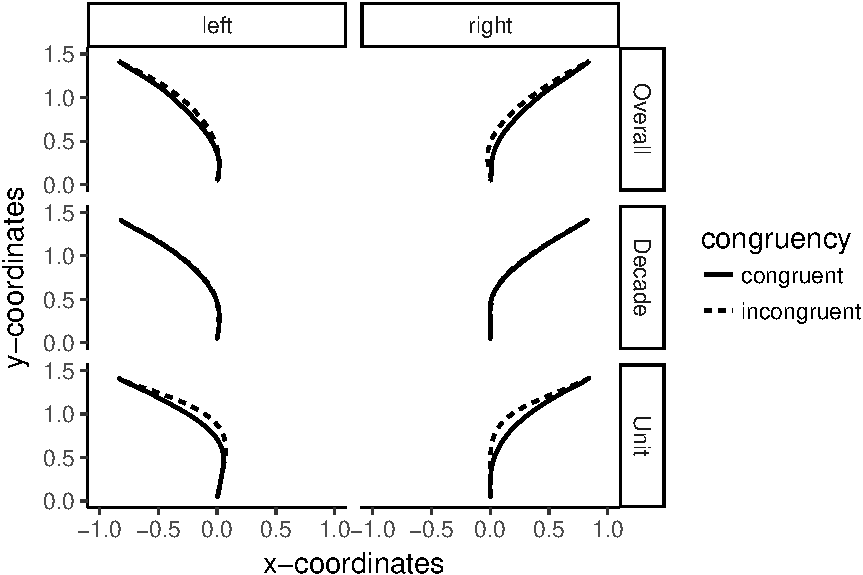
\includegraphics{paper_files/figure-latex/magnitudeTrajectories-1.pdf}
\caption{\label{fig:magnitudeTrajectories}Average normalized mouse
trajectories for the magnitude task, presented as a function of
congruency (congruent, incongruent), instruction condition (overall,
decade only, unit only), and response side (left, right).}
\end{figure}

\begin{figure}
\centering
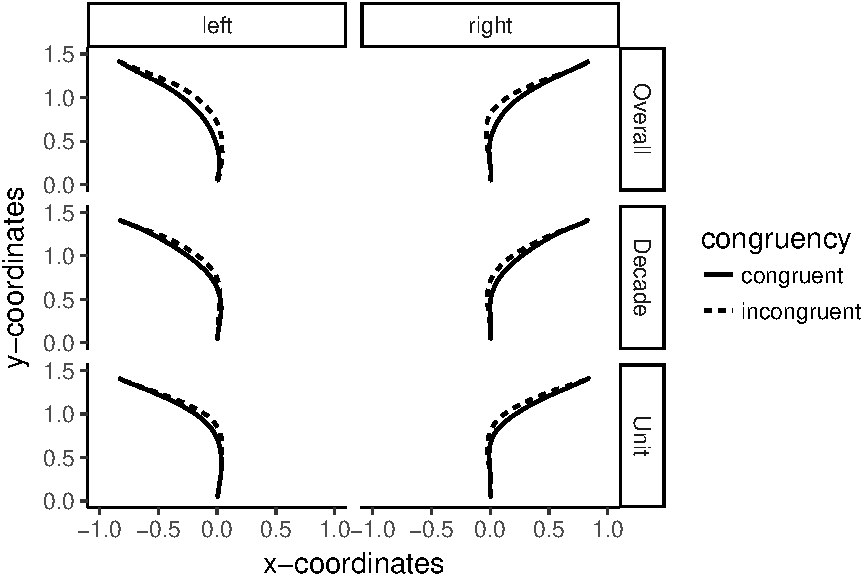
\includegraphics{paper_files/figure-latex/parityTrajectories-1.pdf}
\caption{\label{fig:parityTrajectories}Average normalized mouse trajectories
for the parity task, presented as a function of congruency (congruent,
incongruent), instruction condition (overall, decade only, unit only),
and response side (left, right).}
\end{figure}

\begin{table}[tbp]
\begin{center}
\begin{threeparttable}
\caption{\label{tab:exp2table-traj}Descriptive statistics for trajectory measures in Experiment 2}
\begin{tabular}{llcccc}
\toprule
 &  & \multicolumn{2}{c}{AUC} & \multicolumn{2}{c}{MD} \\
\cmidrule(r){3-4} \cmidrule(r){5-6}
Condition & \multicolumn{1}{c}{Congruency} & \multicolumn{1}{c}{Mean} & \multicolumn{1}{c}{SD} & \multicolumn{1}{c}{Mean} & \multicolumn{1}{c}{SD}\\
\midrule
{\it Magnitude task} &  &  &  &  & \\
Overall & congruent & 0.40 & 0.77 & 0.25 & 0.37\\
 & incongruent & 0.56 & 0.91 & 0.33 & 0.41\\
Decade & congruent & 0.52 & 0.89 & 0.32 & 0.40\\
 & incongruent & 0.51 & 0.85 & 0.32 & 0.39\\
Unit & congruent & 0.65 & 0.99 & 0.38 & 0.44\\
 & incongruent & 0.89 & 1.11 & 0.49 & 0.48\\
{\it Parity task} &  &  &  &  & \\
Overall & congruent & 0.59 & 0.91 & 0.35 & 0.41\\
 & incongruent & 0.81 & 1.07 & 0.46 & 0.46\\
Decade & congruent & 0.65 & 1.03 & 0.38 & 0.43\\
 & incongruent & 0.82 & 1.12 & 0.45 & 0.46\\
Unit & congruent & 0.80 & 1.09 & 0.44 & 0.47\\
 & incongruent & 0.96 & 1.17 & 0.51 & 0.48\\
\bottomrule
\addlinespace
\end{tabular}
\begin{tablenotes}[para]
\textit{Note.} AUC = area under curve; MD = maximum deviation.
\end{tablenotes}
\end{threeparttable}
\end{center}
\end{table}

To see how the magnitude and parity decisions unfolded over time, we
plotted average mouse trajectories as a function of congruency and
instruction condition. Trajectories for the magnitude task are depicted
in Figure \ref{fig:magnitudeTrajectories}, and trajectories for the
parity task are depicted in Figure \ref{fig:parityTrajectories}.

\begin{figure}
\centering
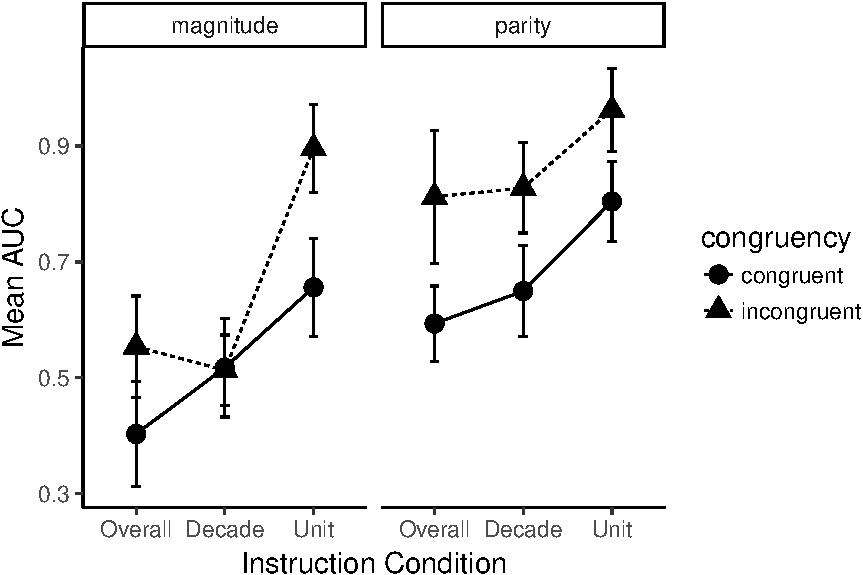
\includegraphics{paper_files/figure-latex/exp2-auc-1.pdf}
\caption{\label{fig:exp2-auc}Mean area-under-the-curve (AUC) values for
Experiment 2, presented as a function of congruency (congruent,
incongruent), instruction condition (overall, decade only, unit only),
and task (magnitude, parity). Error bars represent within-subject 95\%
confidence intervals as recommended by Morey (2008).}
\end{figure}

As with our other dependent measures, we tested how the congruency
effect (as manifested in trajectory curvatures) differed between the
three instructional conditions. Recall that curvature is numerically
indexed by two measures: AUC (area under the curve) and MD (maximum
deviation). Summary statistics for AUC and MD can be seen in Table
\ref{tab:exp2table-traj}. Since the pattern of results did not differ
between AUC and MD, we report only the results for AUC. We first
submitted mean AUCs for participants in the overall condition to a
two-way ANOVA with independent variables of task and congruency. As can
be seen in Figure \ref{fig:exp2-auc}, we observed a significant main
effect of task, \(F(1, 18) = 10.89\), \(p = .004\), \(\eta^2_p = .377\),
indicating that curvatures in the parity task were greater than those in
the magnitude task. There was also a significant main effect of
congruency, \(F(1, 18) = 59.54\), \(p < .001\), \(\eta^2_p = .768\),
where curvatures for incongruent numbers were greater than curvatures
for congruent numbers. The interaction between task and congruency was
not statistically significant, \(F(1, 18) = 2.52\), \(p = .130\),
\(\eta^2_p = .123\).

Next we submitted mean AUCs in the decade-only and unit-only conditions
to a three-way ANOVA with independent variables of task, congruency, and
instructional condition. There was a significant main effect of
instruction, \(F(1, 38) = 5.00\), \(p = .031\), \(\eta^2_p = .116\),
indicating that curvatures in the unit-only condition were greater than
those in the decade-only condition. There was also a significant main
effect of congruency, \(F(1, 38) = 40.46\), \(p < .001\),
\(\eta^2_p = .516\), where curvatures for incongruent numbers were
greater than curvatures for congruent numbers. There was also a main
effect of task, \(F(1, 38) = 20.98\), \(p < .001\), \(\eta^2_p = .356\),
reflecting greater curvatures for the parity task than for the magnitude
task.

Further, we observed a significant interaction between congruency and
instruction, \(F(1, 38) = 6.21\), \(p = .017\), \(\eta^2_p = .141\), and
this interaction depended on task, as signified by a significant
three-way interaction, \(F(1, 38) = 26.86\), \(p < .001\),
\(\eta^2_p = .414\). As shown in Figure \ref{fig:exp2-auc}, participants
who were asked to focus only on the decade digit and ignore the unit
digit exhibited no effect of congruency on AUCs in the magnitude task,
\(t(19) = -0.15\), \(p = .885\). However, as we observed with RTs (in
Experiment 1) and MTs (in Experiment 2), we did observe a large
congruency effect in the parity task, \(t(19) = 4.78\), \(p < .001\).
Finally, when participants were asked to pay attention to only the units
digit, a large congruency effect appeared in both the magnitude task,
\(t(19) = 5.30\), \(p < .001\), and the parity task, \(t(19) = 4.99\),
\(p < .001\). No other terms in the ANOVA model were statistically
significant.

\subsection{Discussion}\label{discussion-1}

Experiment 2 provides further evidence that varying task instructions
may cause participants to modulate their focus of attention to the
surrounding digits, depending on their respective relevance for accurate
task completion. As in Experiment 1, the overall condition yielded
similar pattern of congruency effects across the two tasks (magnitude
and parity). But, different patterns occurred when participants were
asked to focus only on one digit. For example, when the task required
magnitude comparison on \emph{unit} targets, participants' mouse
trajectories were initially biased towards the irrelevant digit in the
decade position, resulting in relatively large reach curvatures and
longer MTs on incongruent compared to congruent trials. In contrast,
when the task required magnitude comparison on \emph{decade} targets,
the absence of curvature and MT differences between congruent and
incongruent trials implies that the reaching movements were immune to
interference from the irrelevant digit in the unit position. On the
other hand, when the task required parity judgment, we observed
interference effects (longer MTs, greater AUCs) with varying strengths
from incongruent primes in both positions, suggesting that irrelevant
digits in both decade and unit positions can bias participants' spatial
attention towards competing response options.

It is perhaps interesting that movement initiation was relatively immune
to our experimental manipulations. However, we did find a small effect
of congruency on initiation times, as well as a trend toward longer
initiation times over the course of overall condition (where
participants focus on the whole digit) as compared to decomposed
conditions (where participants focus on a single component). The
differences in initiation times suggest that the speed with which a
response was initiated may have been influenced by perceptual complexity
of the stimulus number. It may be the case that target digits with
longer length (i.e., two digits versus a single digit) might increase
perceptual load, which in turn increases the time for response
initiation. This interpretation of the data would be consistent with
previous research indicating that initiation time and reach curvature
originate from two dissociable processes (e.g., Erb, Moher, Sobel, \&
Song, 2016; Ruitenberg et al., 2016; Strauss, Woodgate, Sami, \& Heinke,
2015). Specifically, it is thought that initiation times might be driven
by an early action planning stage that is tied to cue-related encoding
processes, whereas MT and AUC might reflect mainly top-down (controlled)
processes which provide for revision and correction of the decision
during the movement execution phase (e.g., Faulkenberry et al., 2016; K.
V. Sobel, Puri, \& Faulkenberry, 2016; Sobel, Puri, Faulkenberry,
\& Dague, 2017). All together, our analysis of movement dynamics echoes
and extends the results obtained using the traditional keypress paradigm
in Experiment 1. Possible implications of these findings for
understanding the time-course of two-digit number representation are
addressed in the General Discussion.

\section{General Discussion}\label{general-discussion}

The aim of the present study was to investigate unit-decade bindings in
two-digit numbers and examine how they are created as function of task
instruction. To this end, we asked participants to perform parity or
magnitude tasks while paying attention to a specific digit (either the
decade digit or the unit digit). Critically, we manipulated congruency
of the irrelevant distractor digit with respect to the specific task. In
the two experiments, participants in the magnitude task experienced a
large degree of interference from an incongruent prime in the decade
digit when asked to pay attention to only the unit digit. On the other
hand, when participants were asked to pay attention to only the decade
digit, no such interference from the incongruent prime in the unit
position was observed. A different pattern emerged in the parity task,
where interference effects from incongruent primes were observed in both
instructional conditions. Thus, changes in task instruction are
sufficient to divert attentional resources to a specific position within
a two-digit number, indicating that (1) people form decomposed
representations of two-digit numbers, and (2) unit-decade binding is not
always obligatory. This finding is consistent with previous research
indicating that the amount of attentional weight given to the processing
of decades or units can be regulated by manipulating task
characteristics (e.g., Castronovo \& Crollen, 2011; Macizo \& Herrera,
2011; Reynvoet et al., 2011). Moreover, such evidence constrains the
syntactic structure model of two-digit numbers which predicts that
compatibility should be mainly affected by numbers' decade digits but
not by numbers' unit digits (Ganor-Stern et al., 2007). All together,
these results, combined with previous studies, suggest that two-digit
number representations are adaptive to manipulations of experimental
context.

The asymmetry of the unit-decade compatibility effects observed in the
present study can be interpreted as a consequence of the dynamic
reorganization of attentional weights that are associated with the
different roles that decades and units play in a given task. For
example, when performing magnitude comparison in two-digit numbers, task
requirements dictate that participants should focus a large portion of
their attention on the decade digit, as the decade must necessarily be
processed in order to perform the comparison task. This increased
attentional weight toward the decade digit apparently persists when
people are asked to focus only on the unit digit. However, when people
are asked to focus only on the decade digit, no such interference
occurs. It is important to stress that the present study goes beyond
previous experiments that examined unit-decade compatibility because
here we show that compatibility between two-digits can emerge even when
participants are asked to pay attention to a single component of a
two-digit number.

Another goal of the present study was to establish the point in the
stimulus processing stream at which the unit-decade conflict first
emerges and how it is resolved over time. We did so by analyzing the
early and late kinematic parameters afforded by computer mouse tracking.
In this analyses, we detected two distinctive influences with
time-varying patterns on response decisions. The first notable influence
appeared in the earliest stages of movement with initiation times.
Specifically, the speed with which participants initiated their hand
movements was influenced by complexity of the string of digits (holistic
vs.~decomposed), but less so by congruency condition. In contrast to
this, the congruency effect from incongruent primes was evident
relatively late in movement, as trajectories showed more attraction
toward the incorrect response option on incongruent than on congruent
trials.

We next discuss the implications of these findings for understanding how
two-digit number processing unfolds over time. One possible explanation
is that the initiation time measure in our study might reflect an early
processing stage at which the identity of the digits is already coded
but not yet assigned to the corresponding unit and decade positions
within the number. Only at a later phase of movement execution, as more
information accumulates, participants start associating digit identities
with a specific position within the number, resulting in increased
attraction of response trajectories toward the incorrect response on
incongruent trials (see Dotan \& Dehaene, 2013 for a similar argument
with number-to-position task). This interpretation of the data fits well
with a dynamic view of decision-making which describes decision process
as a continuous competition between response alternatives in which
initial choice can be revised at any time during the movement as soon as
new information becomes available (Spivey et al., 2005). This
explanation would also be consistent with earlier findings favoring a
distinction between effects of action planning and online control (Erb
et al., 2016; Ruitenberg et al., 2016; Strauss et al., 2015).

Moreover, our findings may provide an empirical validation for recent
conceptual distinction introduced by Nuerk, Moeller, and Willmes (2014)
assuming that the place-value system for multi-digit numbers is
subserved by different steps. A first step, place-identification, refers
to the earliest stages of perceptual encoding at which relevant symbols
(Arabic digits) are differentiated based on their positional identity
(i.e., units, tens, etc), without activating their corresponding
semantic values. At the subsequent step, place-value activation, the
semantic values associated with those digit positions become activated,
leading to the empirically observed compatibility effect. A third step,
place-value computation, is recruited in particular situations when
place-value properties are required to solve a multi-digit arithmetic
task, and thus is not relevant for the present discussion. The
difference found between early and late measures of mouse movement is
consistent with the above suggestion that early visual identification
processing -- at least in part -- precedes the position coding processes
that takes place later and causes the congruency effect. One possible
reason for this is that place-value coding relies on availability of
binding and maintenance processes in working memory, which takes more
time to retrieve, thereby, cascading it to later stages of processing.
Another possibility is that competition between response alternatives
takes place only when overt response starts, thus becoming visible only
during a response-related stage of processing. Further research is
needed to disentangle between these alternative possibilities.

Next, we provide a theoretical framework to explain how task
instructions may modulate unit-decade binding in two-digit number
comparison. For this purpose, we use a variant of dual-route model that
has been shown to account for a number of key findings in the number
domain, such as the SNARC effect and the size congruity effect (Gevers,
Verguts, Reynvoet, Caessens, \& Fias, 2006; Santens et al., 2011).
According to this model, congruity effects originate from parallel
activation of two independently operating routes that interact at the
decision level. The first (unconditional) route automatically processes
task-irrelevant stimulus information and primes the associated response,
while the second (conditional) route codes for task-relevant stimulus
information and is activated intentionally on basis of task
instructions. Changing the instructions (task-related route) leads to a
change in the pattern of weights that determine which stimulus features
are bound to response features. The functional differences between the
mapping of relevant and irrelevant stimulus features to responses (on
the basis of instructions) is sufficient to create different types of
congruency. To see this, suppose that a task entails a magnitude
comparison of the unit digit only. Participants are then presented with
stimulus \enquote{78}, for which (in this specific task) decade places
are irrelevant. In this case, both routes (conditional and
unconditional) activate the same response, since with a compatible
number like \enquote{78}, both digits are larger than referent value of
5. The result is that a response is executed relatively quickly.
However, when a new task instruction is given emphasizing parity
judgment, pre-existing links between stimulus features and responses are
re-bound to form a new meaning. More specifically, now both routes
converge on opposing responses, as now \enquote{78} is an incompatible
number, since the two digits have opposite parity status. The result
here is that RTs are increased. The main point is that the proposed
model accounts for two key characteristics responsible for the
compatibility effect in our study: namely, the modulatory effects of
instructions and its response-related origin. However, to account for
the observed asymmetry in our data, the model needs to make additional
assumptions with respect to how strongly the dominant stimulus values
(decades or units) are associated with response options (magnitude or
parity) such that the gradient of connections is increasing to one of
the response labels but decreasing to the other.

Finally, we discuss some possible limitations of our study. First,
despite the efforts to achieve comparability by applying the same
stimulus sets and mostly equivalent procedural details to parity and
magnitude tasks, the present study does not rule out a potential
contribution of mechanistic differences between these two tasks. At
least in the context of the SNARC effect, previous researchers have
pointed out that parity and magnitude judgment are not equivalent with
respect to working memory resources (Herrera, Macizo, \& Semenza, 2008;
van Dijck, Gevers, \& Fias, 2009). Additionally, it could be argued that
in situations where subjects shift between tasks, the history of
previous experience with, for example, a magnitude comparison task, may
remain active and later interfere with a new task goal of judging
parity. Under these circumstances, it is unclear whether the observed
pattern of interference effects are driven by activation of the current
or previously seen context when switching between two tasks (Kiesel et
al., 2010; Vandierendonck, Liefooghe, \& Verbruggen, 2010). To
counteract for such task-transition effects, we further validated our
methodological approach in Experiment 2 by manipulating the instruction
assignment for the magnitude comparison and parity-judgment tasks
\emph{between} rather than within subjects. This procedure helped to
ensure that distractor category conflicted with the target category on
only one dimension of task context (i.e., whether the task was parity or
magnitude). The results of Experiment 2 were largely similar to those of
Experiment 1, providing further evidence that components of a two-digit
number become bound due to instructional context rather than via an
\emph{a priori} representational binding.

Note also that in our experiment we varied task instruction by
specifically asking participants to process the presented two-digit
numbers in a task-defined manner. This instructional manipulation is
\emph{imperative}; participants must attend to specific digits in order
to successfully complete the task without error. As such, our experiment
is not exactly the same as an \emph{emphasis} manipulation, where the
attentional weight of the units or decades is selectively varied. In our
discussions throughout this manuscript, we have addressed the
possibility that our observed performance patterns are due to the
changing of attentional weights; at present, this is purely speculative.
A stronger case could be made in future work if one could study the role
of varying attentional weights directly, either by manipulating
selectivity of attention (Logan, Taylor, \& Etherton, 1996) or intensity
of attention (Steinborn, Langner, \& Huestegge, 2016).

To summarize, our study demonstrates the impact of task instructions for
unit-decade binding in two-digit number representation. We have
demonstrated that processing both components of two-digit numbers is
obligatory only if participants have been asked to consider the
two-digit number as an integral mathematical whole. However, if
participants have been explicitly asked to pay attention to one digit
only, their ability to ignore the irrelevant adjacent digit depends on
the task requirements. This asymmetrical pattern in selective attention
indicates the deep involvement of top-down processes in two-digit number
representation.

\section{Compliance with ethical
standards}\label{compliance-with-ethical-standards}

\paragraph{Conflict of interest}\label{conflict-of-interest}

The authors declare that they have no conflict of interest.

\paragraph{Ethical approval}\label{ethical-approval}

All procedures performed in studies involving human participants were in
accordance with the ethical standards of the institutional and/or
national research committees and with the 1964 Helsinki declaration and
its later amendments or comparable ethical standards.

\paragraph{Informed consent}\label{informed-consent}

Informed consent was obtained from all individual participants included
in the study.

\newpage

\section{References}\label{references}

\setlength{\parindent}{-0.5in} \setlength{\leftskip}{0.5in}

\hypertarget{refs}{}
\hypertarget{ref-castronovo2011}{}
Castronovo, J., \& Crollen, V. (2011). Numerical comparison of two-digit
numbers: How differences at encoding can involve differences in
processing. \emph{Journal of Cognitive Psychology}, \emph{23}(1), 8--17.
doi:\href{https://doi.org/10.1080/20445911.2011.445985}{10.1080/20445911.2011.445985}

\hypertarget{ref-cohenKdoshay2007}{}
Cohen-Kdoshay, O., \& Meiran, N. (2007). The representation of
instructions in working memory leads to autonomous response activation:
Evidence from the first trials in the flanker paradigm. \emph{The
Quarterly Journal of Experimental Psychology}, \emph{60}(8), 1140--1154.
doi:\href{https://doi.org/10.1080/1747021060089674}{10.1080/1747021060089674}

\hypertarget{ref-deJong1994}{}
De Jong, R., Liang, C.-C., \& Lauber, E. (1994). Conditional and
unconditional automaticity: A dual-process model of effects of spatial
stimulus-response correspondence. \emph{Journal of Experimental
Psychology: Human Perception and Performance}, \emph{20}(4), 731--750.
doi:\href{https://doi.org/10.1037/0096-1523.20.4.731}{10.1037/0096-1523.20.4.731}

\hypertarget{ref-dehaene1990}{}
Dehaene, S., Dupoux, E., \& Mehler, J. (1990). Is numerical comparison
digital? Analogical and symbolic effects in two-digit number comparison.
\emph{Journal of Experimental Psychology: Human Perception and
Performance}, \emph{16}(3), 626--641.
doi:\href{https://doi.org/10.1037/0096-1523.16.3.626}{10.1037/0096-1523.16.3.626}

\hypertarget{ref-dewolf2014}{}
DeWolf, M., Grounds, M. A., Bassok, M., \& Holyoak, K. J. (2014).
Magnitude comparison with different types of rational numbers.
\emph{Journal of Experimental Psychology: Human Perception and
Performance}, \emph{40}(1), 71--82.
doi:\href{https://doi.org/10.1037/a0032916}{10.1037/a0032916}

\hypertarget{ref-dotan2013}{}
Dotan, D., \& Dehaene, S. (2013). How do we convert a number into a
finger trajectory? \emph{Cognition}, \emph{129}(3), 512--529.
doi:\href{https://doi.org/10.1016/j.cognition.2013.07.007}{10.1016/j.cognition.2013.07.007}

\hypertarget{ref-erb2016}{}
Erb, C. D., Moher, J., Sobel, D. M., \& Song, J.-H. (2016). Reach
tracking reveals dissociable processes underlying cognitive control.
\emph{Cognition}, \emph{152}, 114--126.
doi:\href{https://doi.org/10.1016/j.cognition.2016.03.015}{10.1016/j.cognition.2016.03.015}

\hypertarget{ref-erb2018}{}
Erb, C. D., Moher, J., Song, J.-H., \& Sobel, D. M. (in press).
Numerical cognition in action: Reaching behavior reveals numerical
distance effects in 5- to 6-year-olds. \emph{Journal of Numerical
Cognition}.

\hypertarget{ref-faulkenberry2014}{}
Faulkenberry, T. J. (2014). Hand movements reflect competitive
processing in numerical cognition. \emph{Canadian Journal of
Experimental Psychology}, \emph{68}(3), 147--151.
doi:\href{https://doi.org/10.1037/cep0000021}{10.1037/cep0000021}

\hypertarget{ref-faulkenberry2016}{}
Faulkenberry, T. J. (2016). Testing a direct mapping versus competition
account of response dynamics in number comparison. \emph{Journal of
Cognitive Psychology}.
doi:\href{https://doi.org/10.1080/20445911.2016.1191504}{10.1080/20445911.2016.1191504}

\hypertarget{ref-faulkenberry2017}{}
Faulkenberry, T. J., Cruise, A., \& Shaki, S. (2017). Reversing the
manual digit bias in two-digit number comparison. \emph{Experimental
Psychology}, \emph{64}(3), 191--204.
doi:\href{https://doi.org/10.1027/1618-3169/a000365}{10.1027/1618-3169/a000365}

\hypertarget{ref-faulkenberryShaki2016}{}
Faulkenberry, T. J., Cruise, A., Lavro, D., \& Shaki, S. (2016).
Response trajectories capture the continuous dynamics of the size
congruity effect. \emph{Acta Psychologica}, \emph{163}, 114--123.
doi:\href{https://doi.org/10.1016/j.actpsy.2015.11.010}{10.1016/j.actpsy.2015.11.010}

\hypertarget{ref-faulkenberry2018}{}
Faulkenberry, T. J., Hartmann, M., \& Witte, M. (in press). Tracking the
continuous dynamics of numerical processing: A brief review and
editorial. \emph{Journal of Numerical Cognition}.

\hypertarget{ref-faulkenberry2015}{}
Faulkenberry, T. J., Montgomery, S. A., \& Tennes, S.-A. N. (2015).
Response trajectories reveal the temporal dynamics of fraction
representations. \emph{Acta Psychologica}, \emph{159}, 100--107.
doi:\href{https://doi.org/10.1016/j.actpsy.2015.05.013}{10.1016/j.actpsy.2015.05.013}

\hypertarget{ref-fischerHartmann2014}{}
Fischer, M. H., \& Hartmann, M. (2014). Pushing forward in embodied
cognition: May we mouse the mathematical mind? \emph{Frontiers in
Psychology}, \emph{5}(1315).
doi:\href{https://doi.org/10.3389/fpsyg.2014.01315}{10.3389/fpsyg.2014.01315}

\hypertarget{ref-freeman2009motions}{}
Freeman, J. B., \& Ambady, N. (2009). Motions of the hand expose the
partial and parallel activation of stereotypes. \emph{Psychological
Science}, \emph{20}(10), 1183--1188.
doi:\href{https://doi.org/10.1111/j.1467-9280.2009.02422.x}{10.1111/j.1467-9280.2009.02422.x}

\hypertarget{ref-freemanAmbady2010}{}
Freeman, J. B., \& Ambady, N. (2010). MouseTracker: Software for
studying real-time mental processing using a computer mouse-tracking
method. \emph{Behavior Research Methods}, \emph{42}(1), 226--241.
doi:\href{https://doi.org/10.3758/BRM.42.1.226}{10.3758/BRM.42.1.226}

\hypertarget{ref-freemanDaleFarmer2011}{}
Freeman, J. B., Dale, R., \& Farmer, T. A. (2011). Hand in motion
reveals mind in motion. \emph{Frontiers in Psychology}, \emph{2}(59).
doi:\href{https://doi.org/10.3389/fpsyg.2011.00059}{10.3389/fpsyg.2011.00059}

\hypertarget{ref-ganorStern2007}{}
Ganor-Stern, D., Tzelgov, J., \& Ellenbogen, R. (2007). Automaticity and
two-digit numbers. \emph{Journal of Experimental Psychology: Human
Perception and Performance}, \emph{33}(2), 483--496.
doi:\href{https://doi.org/10.1037/0096-1523.33.2.483}{10.1037/0096-1523.33.2.483}

\hypertarget{ref-gevers2006}{}
Gevers, W., Verguts, T., Reynvoet, B., Caessens, B., \& Fias, W. (2006).
Numbers and space: A computational model of the SNARC effect.
\emph{Journal of Experimental Psychology: Human Perception and
Performance}, \emph{32}(1), 32--44.
doi:\href{https://doi.org/10.1037/0096-1523.32.1.32}{10.1037/0096-1523.32.1.32}

\hypertarget{ref-herrera2008}{}
Herrera, A., Macizo, P., \& Semenza, C. (2008). The role of working
memory in the association between number magnitude and space. \emph{Acta
Psychologica}, \emph{128}(2), 225--237.
doi:\href{https://doi.org/10.1016/j.actpsy.2008.01.002}{10.1016/j.actpsy.2008.01.002}

\hypertarget{ref-hinrichs1981}{}
Hinrichs, J. V., Yurko, D. S., \& Hu, J.-m. (1981). Two-digit number
comparison: Use of place information. \emph{Journal of Experimental
Psychology: Human Perception and Performance}, \emph{7}(4), 890--901.
doi:\href{https://doi.org/10.1037/0096-1523.7.4.890}{10.1037/0096-1523.7.4.890}

\hypertarget{ref-kallai2012}{}
Kallai, A. Y., \& Tzelgov, J. (2012). The place-value of a digit in
multi-digit numbers is processed automatically. \emph{Journal of
Experimental Psychology: Learning, Memory, and Cognition}, \emph{38}(5),
1221--1233.
doi:\href{https://doi.org/10.1037/a0027635}{10.1037/a0027635}

\hypertarget{ref-kiesel2010}{}
Kiesel, A., Steinhauser, M., Wendt, M., Falkenstein, M., Jost, K.,
Philipp, A. M., \& Koch, I. (2010). Control and interference in task
switching: A review. \emph{Psychological Bulletin}, \emph{136}(5), 849.

\hypertarget{ref-klein2013}{}
Klein, E., Bahnmueller, J., Mann, A., Pixner, S., Kaufmann, L., Nuerk,
H.-C., \& Moeller, K. (2013). Language influences on numerical
development Inversion effects on multi-digit number processing.
\emph{Frontiers in Psychology}, \emph{4}, 480.
doi:\href{https://doi.org/10.3389/fpsyg.2013.00480}{10.3389/fpsyg.2013.00480}

\hypertarget{ref-kornblum1990}{}
Kornblum, S., Hasbroucq, T., \& Osman, A. (1990). Dimensional overlap:
Cognitive basis for stimulus-response compatibility -- A model and
taxonomy. \emph{Psychological Review}, \emph{97}(2), 253--270.
doi:\href{https://doi.org/10.1037/0033-295x.97.2.253}{10.1037/0033-295x.97.2.253}

\hypertarget{ref-liefooghe2013}{}
Liefooghe, B., De Houwer, J., \& Wenke, D. (2013). Instruction-based
response activation depends on task preparation. \emph{Psychonomic
Bulletin \& Review}, \emph{20}(3), 481--487.
doi:\href{https://doi.org/10.3758/s13423-013-0374-7}{10.3758/s13423-013-0374-7}

\hypertarget{ref-logan1996}{}
Logan, G. D., Taylor, S. E., \& Etherton, J. L. (1996). Attention in the
acquisition and expression of automaticity. \emph{Journal of
Experimental Psychology: Learning, Memory, and Cognition}, \emph{22}(3),
620--638.
doi:\href{https://doi.org/10.1037/0278-7393.22.3.620}{10.1037/0278-7393.22.3.620}

\hypertarget{ref-macizo2011}{}
Macizo, P., \& Herrera, A. (2011). Cognitive control in number
processing: Evidence from the unitdecade compatibility effect.
\emph{Acta Psychologica}, \emph{136}(1), 112--118.
doi:\href{https://doi.org/10.1016/j.actpsy.2010.10.008}{10.1016/j.actpsy.2010.10.008}

\hypertarget{ref-macizo2010}{}
Macizo, P., Herrera, A., Paolieri, D., \& Román, P. (2010). Is there
cross-language modulation when bilinguals process number words?
\emph{Applied Psycholinguistics}, \emph{31}(04), 651--669.
doi:\href{https://doi.org/10.1017/s0142716410000184}{10.1017/s0142716410000184}

\hypertarget{ref-moeller2013}{}
Moeller, K., Klein, E., Nuerk, H.-C., \& Willmes, K. (2013). Magnitude
representation in sequential comparison of two-digit numbers is not
holistic either. \emph{Cognitive Processing}, \emph{14}(1), 51--62.
doi:\href{https://doi.org/10.1007/s10339-012-0535-z}{10.1007/s10339-012-0535-z}

\hypertarget{ref-moeller2009}{}
Moeller, K., Nuerk, H.-C., \& Willmes, K. (2009). Internal number
magnitude representation is not holistic, either. \emph{European Journal
of Cognitive Psychology}, \emph{21}(5), 672--685.
doi:\href{https://doi.org/10.1080/09541440802311899}{10.1080/09541440802311899}

\hypertarget{ref-morey2008}{}
Morey, R. D. (2008). Confidence intervals from normalized data: A
correction to cousineau (2005). \emph{Tutorial in Quantitative Methods
for Psychology}, \emph{4}(2), 61--64.

\hypertarget{ref-moyer1967}{}
Moyer, R. S., \& Landauer, T. K. (1967). Time required for judgements of
numerical inequality. \emph{Nature}, \emph{215}(5109), 1519--1520.
doi:\href{https://doi.org/10.1038/2151519a0}{10.1038/2151519a0}

\hypertarget{ref-mussolin2008}{}
Mussolin, C., \& Noël, M.-P. (2008). Automaticity for numerical
magnitude of two-digit arabic numbers in children. \emph{Acta
Psychologica}, \emph{129}(2), 264--272.
doi:\href{https://doi.org/10.1016/j.actpsy.2008.08.001}{10.1016/j.actpsy.2008.08.001}

\hypertarget{ref-nuerk2005}{}
Nuerk, H.-C., \& Willmes, K. (2005). On the magnitude representations of
two-digit numbers. \emph{Psychology Science}, \emph{47}(1), 52--72.

\hypertarget{ref-nuerk2005power}{}
Nuerk, H.-C., Bauer, F., Krummenacher, J., Heller, D., \& Willmes, K.
(2005). The power of the mental number line: How the magnitude of
unattended numbers affects performance in an eriksen task.
\emph{Psychology Science}, \emph{47}(1), 34--50.

\hypertarget{ref-nuerk2014chapter}{}
Nuerk, H.-C., Moeller, K., \& Willmes, K. (2014). Multi-digit Number
Processing. In R. Cohen Kadosh \& A. Dowker (Eds.), \emph{The Oxford
Handbook of Numerical Cognition} (pp. 106--139).
doi:\href{https://doi.org/10.1093/oxfordhb/9780199642342.013.021}{10.1093/oxfordhb/9780199642342.013.021}

\hypertarget{ref-nuerk2011}{}
Nuerk, H.-C., Moeller, K., Klein, E., Willmes, K., \& Fischer, M. H.
(2011). Extending the mental number line. \emph{Zeitschrift Für
Psychologie}, \emph{219}(1), 3--22.
doi:\href{https://doi.org/10.1027/2151-2604/a000041}{10.1027/2151-2604/a000041}

\hypertarget{ref-nuerk2001}{}
Nuerk, H.-C., Weger, U., \& Willmes, K. (2001). Decade breaks in the
mental number line? Putting the tens and units back in different bins.
\emph{Cognition}, \emph{82}(1), B25--B33.
doi:\href{https://doi.org/10.1016/s0010-0277(01)00142-1}{10.1016/s0010-0277(01)00142-1}

\hypertarget{ref-nuerk2005language}{}
Nuerk, H.-C., Weger, U., \& Willmes, K. (2005). Language effects in
magnitude comparison: Small, but not irrelevant. \emph{Brain and
Language}, \emph{92}(3), 262--277.
doi:\href{https://doi.org/10.1016/j.bandl.2004.06.107}{10.1016/j.bandl.2004.06.107}

\hypertarget{ref-ratinckx2005}{}
Ratinckx, E., Brysbaert, M., \& Fias, W. (2005). Naming two-digit Arabic
numerals: Evidence from masked priming studies. \emph{Journal of
Experimental Psychology: Human Perception and Performance},
\emph{31}(5), 1150--1163.
doi:\href{https://doi.org/10.1037/0096-1523.31.5.1150}{10.1037/0096-1523.31.5.1150}

\hypertarget{ref-reynvoet2011}{}
Reynvoet, B., Notebaert, K., \& Van den Bussche, E. (2011). The
processing of two-digit numbers depends on task instructions.
\emph{Zeitschrift Für Psychologie}, \emph{219}(1), 37--41.
doi:\href{https://doi.org/10.1027/2151-2604/a000044}{10.1027/2151-2604/a000044}

\hypertarget{ref-ruitenberg2016}{}
Ruitenberg, M. F. L., Duthoo, W., Santens, P., Seidler, R. D.,
Notebaert, W., \& Abrahamse, E. L. (2016). Sequence learning in
parkinson's disease: Focusing on action dynamics and the role of
dopaminergic medication. \emph{Neuropsychologia}, \emph{93}, 30--39.
doi:\href{https://doi.org/10.1016/j.neuropsychologia.2016.09.027}{10.1016/j.neuropsychologia.2016.09.027}

\hypertarget{ref-santens2011}{}
Santens, S., Goossens, S., \& Verguts, T. (2011). Distance in motion:
Response trajectories reveal the dynamics of number comparison.
\emph{PloS One}, \emph{6}(9), e25429.
doi:\href{https://doi.org/10.1371/journal.pone.0025429}{10.1371/journal.pone.0025429}

\hypertarget{ref-sobel2016}{}
Sobel, K. V., Puri, A. M., \& Faulkenberry, T. J. (2016). Bottom-up and
top-down attentional contributions to the size congruity effect.
\emph{Attention, Perception, \& Psychophysics}, \emph{78}(5),
1324--1336.
doi:\href{https://doi.org/10.3758/s13414-016-1098-3}{10.3758/s13414-016-1098-3}

\hypertarget{ref-sobel2017}{}
Sobel, K. V., Puri, A. M., Faulkenberry, T. J., \& Dague, T. D. (2017).
Visual search for conjunctions of physical and numerical size shows that
they are processed independently. \emph{Journal of Experimental
Psychology: Human Perception and Performance}, \emph{43}(3), 444--453.
doi:\href{https://doi.org/10.1037/xhp0000323}{10.1037/xhp0000323}

\hypertarget{ref-songNakayama2008}{}
Song, J.-H., \& Nakayama, K. (2008). Numeric comparison in a
visually-guided manual reaching task. \emph{Cognition}, \emph{106}(2),
994--1003.
doi:\href{https://doi.org/10.1016/j.cognition.2007.03.014}{10.1016/j.cognition.2007.03.014}

\hypertarget{ref-spivey2005}{}
Spivey, M. J., Grosjean, M., \& Knoblich, G. (2005). Continuous
attraction toward phonological competitors. \emph{Proceedings of the
National Academy of Sciences}, \emph{102}(29), 10393--10398.
doi:\href{https://doi.org/10.1073/pnas.0503903102}{10.1073/pnas.0503903102}

\hypertarget{ref-steinborn2016}{}
Steinborn, M. B., Langner, R., \& Huestegge, L. (2016). Mobilizing
cognition for speeded action: Try-harder instructions promote motivated
readiness in the constant-foreperiod paradigm. \emph{Psychological
Research}, \emph{81}(6), 1135--1151.
doi:\href{https://doi.org/10.1007/s00426-016-0810-1}{10.1007/s00426-016-0810-1}

\hypertarget{ref-strauss2015}{}
Strauss, S., Woodgate, P. J., Sami, S. A., \& Heinke, D. (2015). Choice
reaching with a LEGO arm robot (CoRLEGO): The motor system guides visual
attention to movement-relevant information. \emph{Neural Networks},
\emph{72}, 3--12.
doi:\href{https://doi.org/10.1016/j.neunet.2015.10.005}{10.1016/j.neunet.2015.10.005}

\hypertarget{ref-vanDijck2009}{}
van Dijck, J.-P., Gevers, W., \& Fias, W. (2009). Numbers are associated
with different types of spatial information depending on the task.
\emph{Cognition}, \emph{113}(2), 248--253.
doi:\href{https://doi.org/10.1016/j.cognition.2009.08.005}{10.1016/j.cognition.2009.08.005}

\hypertarget{ref-vandierendonck2010}{}
Vandierendonck, A., Liefooghe, B., \& Verbruggen, F. (2010). Task
switching: Interplay of reconfiguration and interference control.
\emph{Psychological Bulletin}, \emph{136}(4), 601.

\hypertarget{ref-verguts2005}{}
Verguts, T., \& De Moor, W. (2005). Two-digit comparison: Decomposed,
holistic, or hybrid? \emph{Experimental Psychology}, \emph{52}(3),
195--200.
doi:\href{https://doi.org/10.1027/1618-3169.52.3.195}{10.1027/1618-3169.52.3.195}

\hypertarget{ref-wenke2005}{}
Wenke, D., \& Frensch, P. A. (2005). The influence of task instruction
on action coding: Constraint setting or direct coding? \emph{Journal of
Experimental Psychology: Human Perception and Performance},
\emph{31}(4), 803--819.
doi:\href{https://doi.org/10.1037/0096-1523.31.4.803}{10.1037/0096-1523.31.4.803}

\hypertarget{ref-wenkeGaschler2005}{}
Wenke, D., Gaschler, R., \& Nattkemper, D. (2005). Instruction-induced
feature binding. \emph{Psychological Research}, \emph{71}(1), 92--106.
doi:\href{https://doi.org/10.1007/s00426-005-0038-y}{10.1007/s00426-005-0038-y}

\hypertarget{ref-zorzi1995}{}
Zorzi, M., \& Umiltà, C. (1995). A computational model of the Simon
effect. \emph{Psychological Research}, \emph{58}(3), 193--205.
doi:\href{https://doi.org/10.1007/bf00419634}{10.1007/bf00419634}






\end{document}
